\chapter{Narukvica}
\label{pog:bracelet}
Svrha narukvice je prikupljanje biomedicinskih parmetara korisnika i njihovo slanje na obradu na glavnoj ploči. Biomedicinski parametri koji će se promatrati su brzina otkucaja srca putem fotopletizmografskog senzora (PPG) i impedancija kože, odnosno elektrodermalna aktivnost. Promjena elektrodermalna aktivnost je dobar pokazatelj stresa u korisnika \cite{edr}, a osobe sa poremećajem tečnosti govora pokazuju značajno smanjenje brzine otkucaja srca u stresnim situacijama u odnosu na osobe bez takvih poremećaja \cite{ALM2004123}.

Što se tiče zahtjeva na napajanje narukvice, situacija je ista kao i kod glavne ploče, uz drugačiju potrošnju. Tako da izrada pločice za narukvicu predstavlja mogućnost ispravljanja grešaka nastalih tijekom dizajna napajanja glavne ploče. Narukvica također mora imati mogućnost bežične komunikacije. S obzirom na ograničenje veličine ploče maknuti su kratkospojnici i testne točke.

\section{Bežična komunikacija}
Shema bežične komunikacije na narukvici (slika \ref{slk:BR_WIRELESS}) je veoma slična onoj na glavnoj ploči (slika \ref{slk:WIFI}), uz nedostatak kratkospojnika, dodatak signala za upravljanje I\textsubscript{2}C sučeljem i korištenje analogno-digitalnog pretvornika za mjerenje impadancije kože. Još jedna promjena dolazi u obliku programiranja preko UART-a. S obzirom na probleme tijekom programiranja glavne ploče dodani su signali DTR i CTS kako bi se BOOT i EN stezaljke ESP mikrokontrolera mogle programski upravljati.
\begin{sidewaysfigure}[htbp]
    \centering
    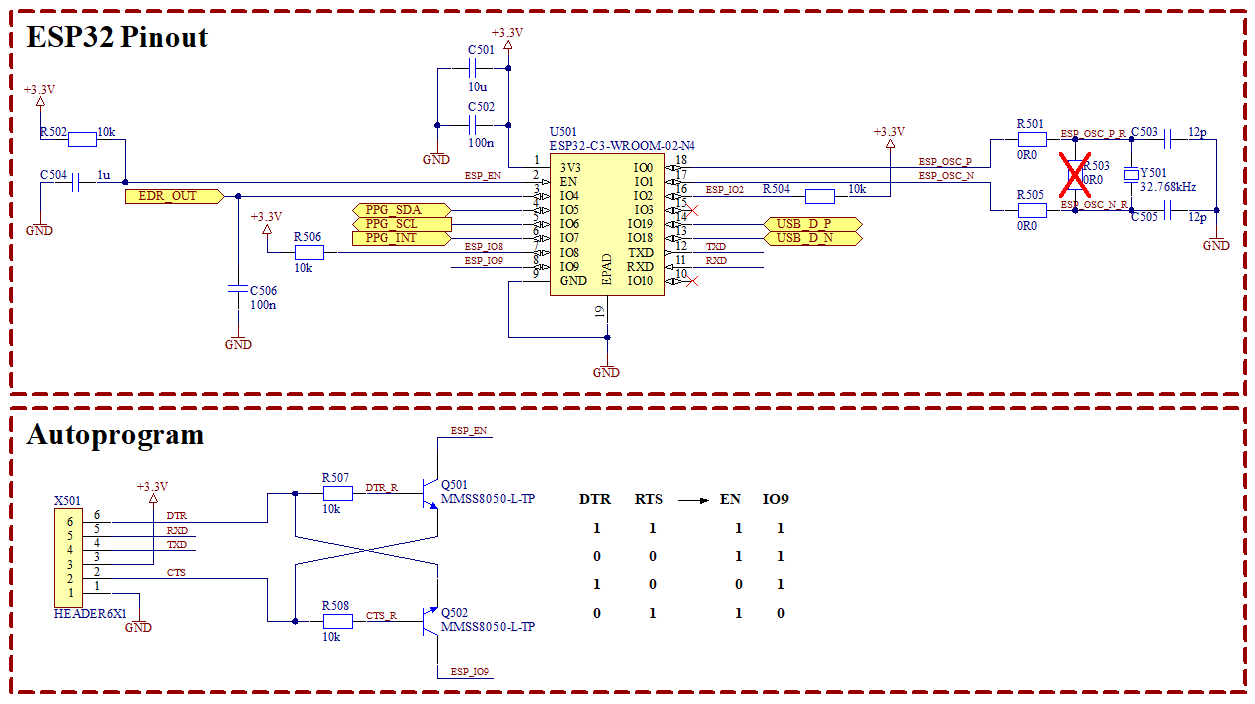
\includegraphics[width=1\textwidth]{Figures/BR_WIRELESS.png}
    \caption{Shema bežične komunikacije narukvice}
    \label{slk:BR_WIRELESS}
\end{sidewaysfigure}

\newpage
\section{Fotopletizmografski senzor}

Za mjerenje brzine otkucaja srca koristi se PPG senzor MAX30101 tvrtke Analog Devices (slika \ref{slk:MAX30101}). Ovaj snezor u sebi ima crvenu, zelenu i infracrvenu svjetleću diodu i fotosenzor, upravljačko sklopovlje za diode, te komunicira preko I\textsuperscript{2}C sučelja. Kao što je vidljivo na shemi na slici \ref{slk:PPG} ovaj senzor je veoma jednostavan za implementaciju uz svega par par priteznih otpornika i blokadnih kondenzatora. Jedina komplikacija dolazi u obliku napajanja od 5 V, koje je potrebno jer je pad napona na zelenoj svjetlećoj diodi specificiran na 3.3 V.
\begin{figure}[htb]
    \centering
    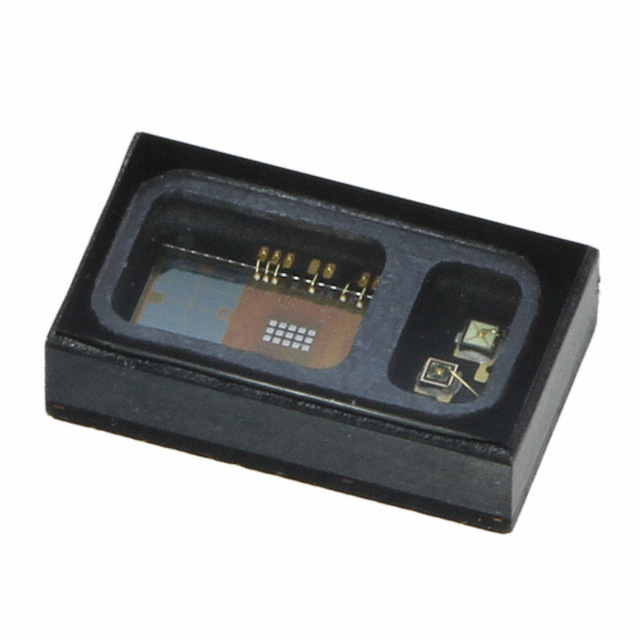
\includegraphics[width=6 cm]{Figures/MAX30101.JPG}
    \caption{MAX30101 PPG senzor}
    \label{slk:MAX30101}
\end{figure}
\begin{figure}[htb]
    \centering
    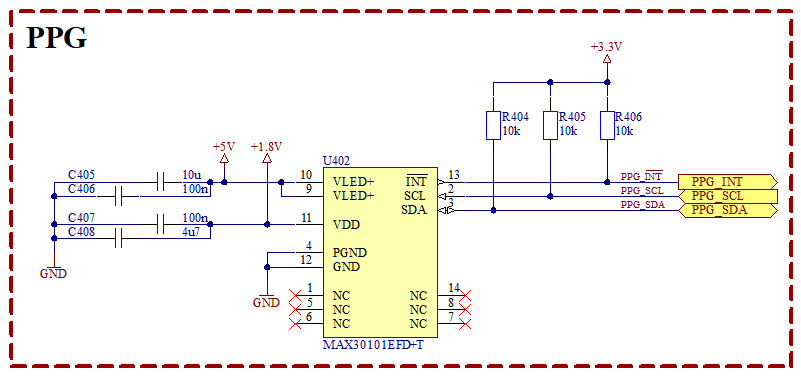
\includegraphics[width=\textwidth]{Figures/PPG.png}
    \caption{Shema PPG senzora}
    \label{slk:PPG}
\end{figure}

\section{Impedancija kože}
Impedancija kože mjerit će se pomoću instrumentacijskog pojačala. Shema mjernog kruga prikazana je na slici \ref{slk:EDR}. Odabrano je instrumentacijsko pojačalo AD8226 tvrtke Analog Devices zbog svog velikog ulaznog otpora, malog šuma i dobrog potiskivanja zajedničkih smetnji \cite{ad:ad8226}. Napajanje pojačala je filtrirano pasivnom mrežom kako ne bi došlo do smetnji od digitalnog dijela sklopovlja.
\begin{figure}[htb]
    \centering
    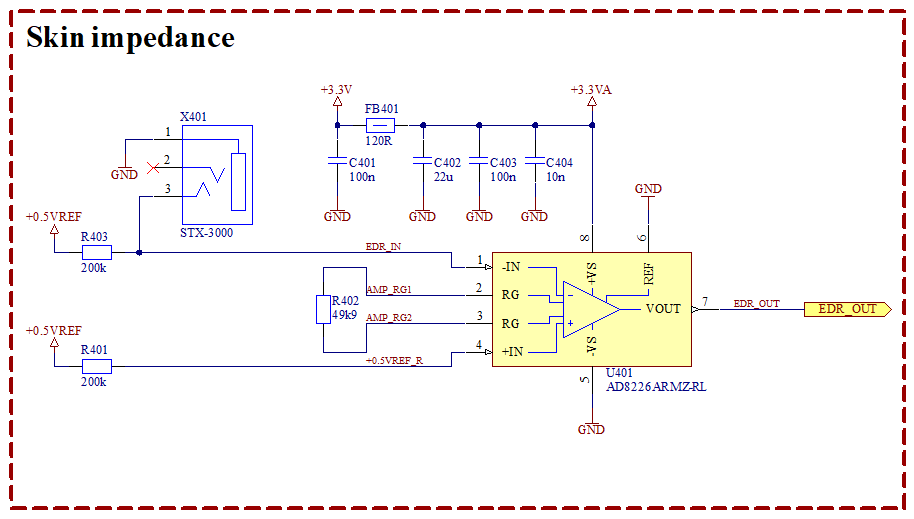
\includegraphics[width=\textwidth]{Figures/EDR.png}
    \caption{Shema mjernog kruga za impedanciju kože}
    \label{slk:EDR}
\end{figure}
Za mjerenje impedancije koristi se referentni napon od 0.5 V, a mjerenje impedancije se temelji na mjerenju napona na naponskom djelilu na stezaljci -IN pojačala. Kožu predstavlja donji otpornik u naponskom djelilu, te razlika između tog napona i referentnog napona pojačava:
\begin{equation} \label{eq:EDR}
    U_{IZ}=A\cdot U_{REF}\cdot \frac{R_{403}}{R_{403}+R_{skin}}
\end{equation}
Impedancija kože mjeri se u stotinama kilooma (maksimalno cca. $250\quad \textrm{k}\Omega$ \cite{rskin}), tako da je vrijednost gornjeg otpornika $200\quad \textrm{k}\Omega$. Pojačanje iznosi 2 i namješta se preko otpornika R402.

Za svrhe lakšeg prototipiranja koristit će se samoljepljive elektrode (slika \ref{slk:ELECTRODE}) koje se montiraju na kabel prikazan na slici \ref{slk:CABLE}. 
\begin{figure}[htb]
    \centering
    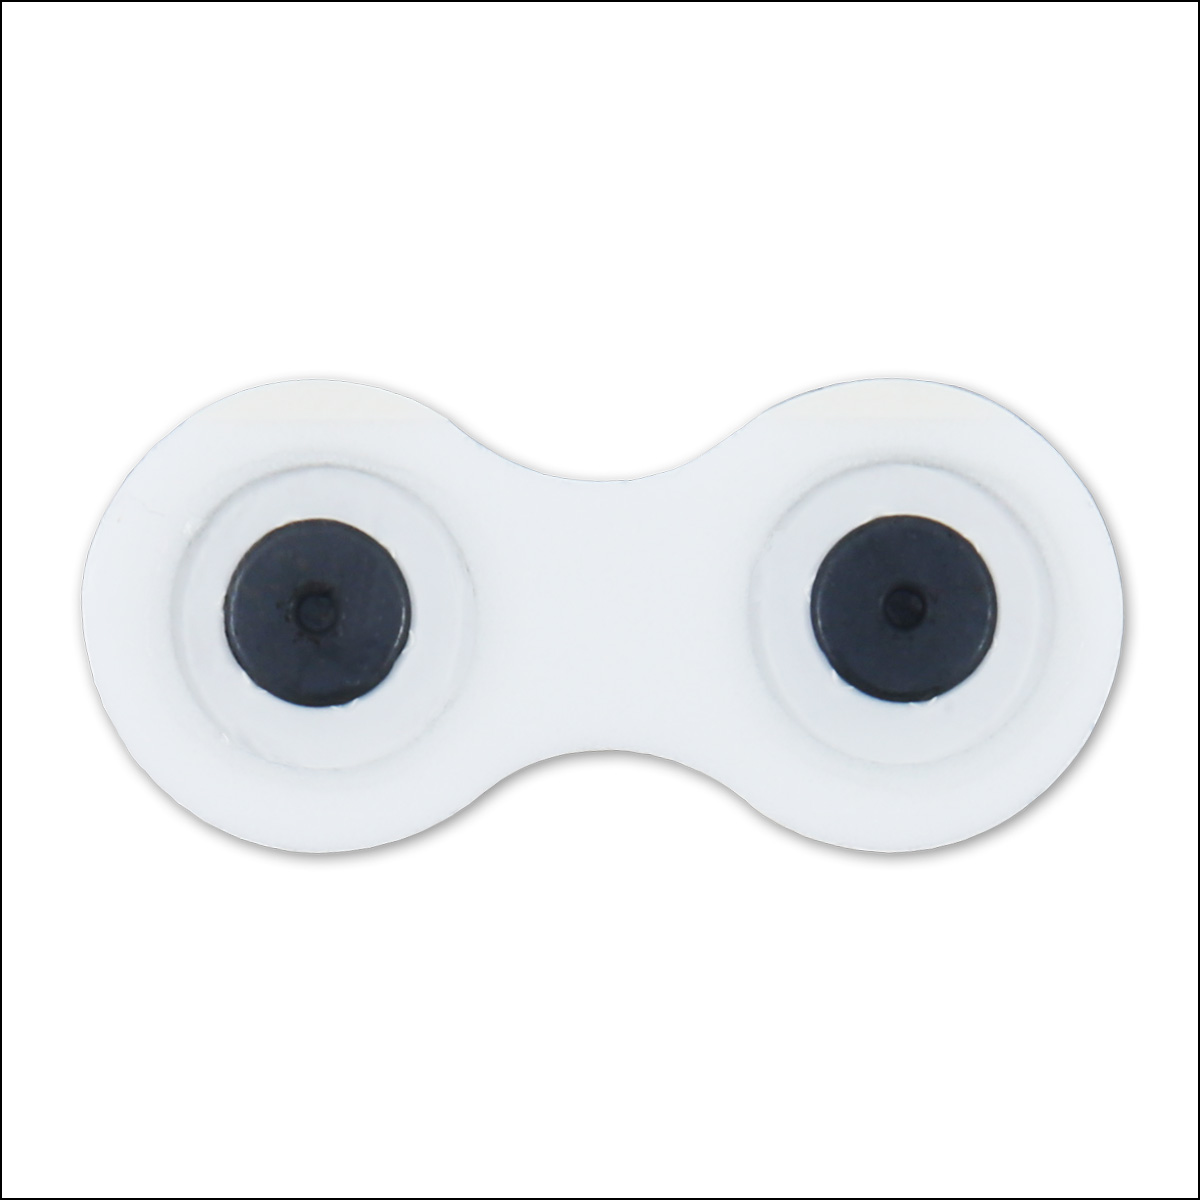
\includegraphics[width=6 cm]{Figures/ELECTRODE-BOTTOM.jpg}
    \caption{Samoljepljiva elektroda}
    \label{slk:ELECTRODE}
\end{figure}
\begin{figure}
    \centering
    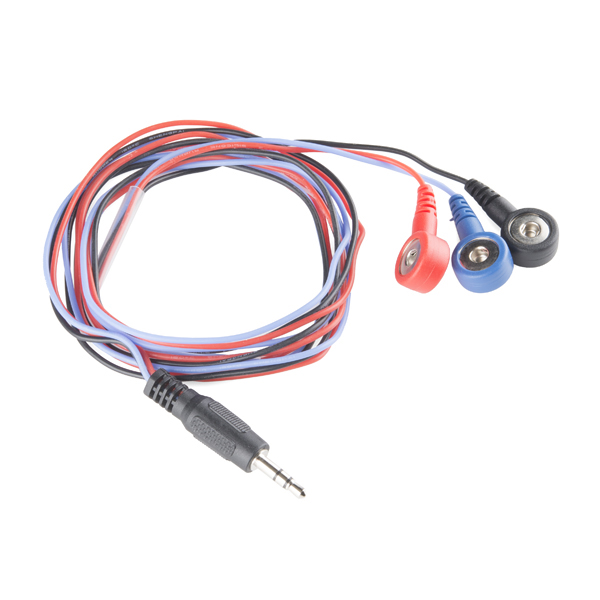
\includegraphics[width=6 cm]{Figures/CABLE.jpg}
    \caption{Kabel za elektrode}
    \label{slk:CABLE}
\end{figure}
Ovaj kabel se spaja na narukvicu putem 3.5 mm audio priključka.

\section{Napajanje}
\subsection{Proračun potrošnje}

Proračun potrošnje za narukvicu je bio puno jednostavniji od proračuna za glavnu ploču. U ovom slučaju, najveći potrošač je i dalje sustav za bežičnu komunikaciju, međutim on je efektivno i jedini potrošać na 3.3 V jer je potrošnja instrumentacijskog pojačala izrazito mala, maksimalno $20\quad \mu \textrm{A}$ \cite{ad:ad8226}. Za potrošnju sustava bežične komunikacije uzima se vrijednost prikazana u tablici \ref{tab:MB3V3}. Na napajanju od 5 V jedini potrošač je PPG senzor i njegova potrošnja u najgorem slučaju iznosi 50 mA, a na napajanju od 1.8 V senzor troši maksimalno 1.1 mA \cite{ad:max30101}.

\subsection{Napajanja od 3.3 V i 1.8 V}
\label{subsec:BR_VDD}
Shema napajanja od 3.3 V i 1.8 V prikazana je na slici \ref{slk:BR_VDD}. U oba slučaja koristi se LDO AP2112K proizvođača Diodes Incorporated. Ovaj LDO je odabran radi svoje male veličine u SOT-25 s obzirom na ograničenje veličine PCB-a. 
\begin{figure}[htb]
    \centering
    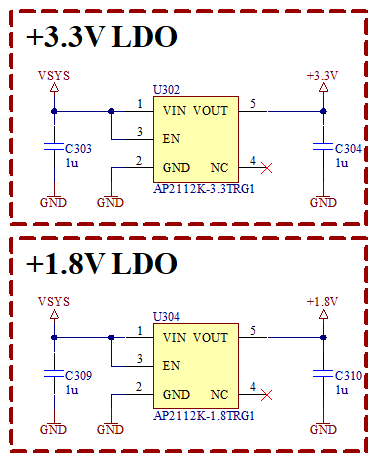
\includegraphics[width=6 cm]{Figures/BR_VDD.png}
    \caption{Napajanje od 3.3 V i 1.8 V za narukvicu}
    \label{slk:BR_VDD}
\end{figure}

\subsection{Referentni napon}

Shema izvora referentnog napona prikazana je na slici \ref{slk:BR_VREF}. Koristi se ADR130 referenca tvrtke Analog Devices. Iznos referentnog napona se može namjestiti na 1 V ili 0.5 V, a veličina kućišta je ista kao i kod linearnih regulatora prikazanih u dijelu \ref{subsec:BR_VDD}.
\begin{figure}[htb]
    \centering
    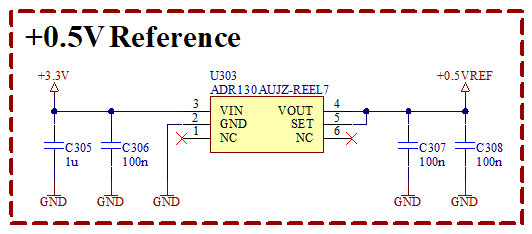
\includegraphics[width=10 cm]{Figures/BR_VREF.png}
    \caption{Referentni izvor napona od 0.5 V}
    \label{slk:BR_VREF}
\end{figure}

\subsection{Napajanje od 5 V}

Za napajanje od 5 V bilo je potrebno dizajnirati uzlazni prekidački regulator. Shema regulatora prikazana je na slici \ref{slk:BR_BOOST}. Odabran je TLV61220 proizvođača Texas Instruments jer je idealan za napajanje sa baterije. Regulator može raditi na ulaznom naponu od 0.7 V do 5.5 V i potrebno je malo komponenata za rad \cite{ti:tlv61220}. Također je pogodan radi svoje male veličine u SOT-23 kućištu.
\begin{figure}[htb]
    \centering
    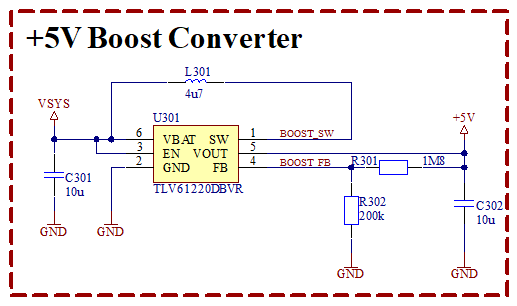
\includegraphics[width=13 cm]{Figures/BR_BOOST.png}
    \caption{Uzlazni prekidački regulator}
    \label{slk:BR_BOOST}
\end{figure}
Zavojnica je odabrana prema preporukama proizvođača, a naponsko djelilo je proračunato imajući na umu da donji otpornik ne bi trebao biti veći od $500\quad \textrm{k}\Omega$ kako bi vrijednost struje koja teče u FB stezaljku bila što bliže $0.01 \quad \mu \textrm{A}$ \cite{ti:tlv61220}.
Efikasnost za izlazne struje od 1 mA do 50 mA je skoro ista na ulaznom naponu u rasponu baterije i može se uzeti efikasnost od 90 \% \ref{slk:BOOST_EFF}. Uz minimalni ulazni napond od 3V, potrošnja, prema jednadžbi \ref{eq:IN_CURR} iznosi 75 mA.
\begin{figure}[htb]
    \centering
    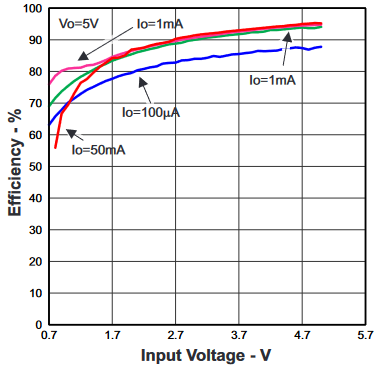
\includegraphics[width=8 cm]{Figures/BOOST_EFF.png}
    \caption{Efikasnost regulatora \cite{ti:tlv61220}}
    \label{slk:BOOST_EFF}
\end{figure}

\section{Punjač}

Uzevši u obzir potršnju svih podsustava ukupna struja koju punjač mora moći dati je 426.12 mA. Uz struju punjenja baterije od 1 A i uzevši u obzir jednadžbe \ref{eq:IN_CURR} i \ref{eq:IN_CURR_MAX} ukupna struja koju USB sučelje mora moći dati iznosi 1.08 A, dakle uzet će se ograničenje na ulaznu struju od 1.5 A. Uvijeti su, dakle, veoma slični onima kod glavne ploče.